To demonstrate the applicability of our design and implementation, we
conduct three case studies.


\noindentparagraph{Type safety of STLCs.}

The first case study is the mechanization of the type safety theorem of
STLC and those of its extensions,
which has been occurring in the examples in this paper.
The code base is ported from Software Foundations~\cite{sf-pl}.
%
The base STLC family consists of about 400 lines of code.
Lines of code in each of the four derived families
($\mathrm{Y}$, $\times$, $+$, and $\mu$ in the Venn diagram)
vary from 100 to 250, largely depending on how many constructors they
add to the inductive types.
%
The linguistic nature of our approach allows us to retain a programming
style similar to the original proofs in Software Foundations.

\begin{wrapfigure}[11]{r}{0.28\textwidth}
\small
\renewcommand*{\arraystretch}{0.75}

\def\CircFix{(135:0.707cm) circle (1.5cm)}
\def\CircProd{(45:0.707cm) circle (1.5cm)}
\def\CircIsorec{(-45:0.707cm) circle (1.5cm)}
\def\CircSum{(-135:0.707cm) circle (1.5cm)}

\definecolor{FixColor}{HTML}{FF9966}
\definecolor{ProdColor}{HTML}{66CCFF}
\definecolor{SumColor}{HTML}{FFFF66}
\definecolor{IsorecColor}{HTML}{FF6699}

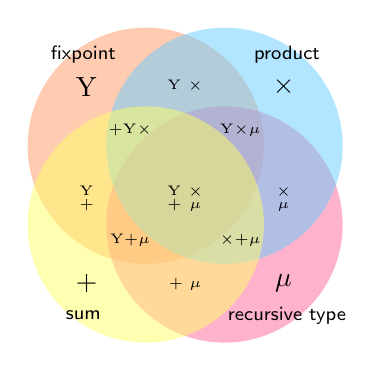
\begin{tikzpicture}
    \begin{scope}[shift={(0cm,-0cm)}, fill opacity=0.50]
        \fill[FixColor] \CircFix;
        \fill[IsorecColor] \CircIsorec;
        \fill[ProdColor] \CircProd;
        \fill[SumColor] \CircSum;
%       \draw \CircFix;
%       \draw \CircIsorec;
%       \draw \CircProd;
%       \draw \CircSum;
    \end{scope}

    \node at (0: 0) {%
        \begin{minipage}{1cm}\tiny
        \[\begin{array}{@{}c@{\ }c@{}}
            \mathrm{Y} & \times\\ + & \mu
        \end{array}\]
        \end{minipage}
    };
    \node at (-180: 1.25cm) {%
        \begin{minipage}{1cm}\tiny
        \[\begin{array}{@{}c@{}}
            \mathrm{Y}\\ +
        \end{array}\]
        \end{minipage}
    };
    \node at (0: 1.25cm) {%
        \begin{minipage}{1cm}\tiny
        \[\begin{array}{@{}c@{}}
            \times\\ \mu
        \end{array}\]
        \end{minipage}
    };
    \node at (90: 1.26cm) {\tiny$\mathrm{Y}\ \times$};
    \node at (-90: 1.26cm) {\tiny$+\ \mu$};
    \node at (135: 1.768cm) {$\mathrm{Y}$};
    \node at (-135: 1.768cm) {$+$};
    \node at (45: 1.768cm) {$\times$};
    \node at (-45: 1.768cm) {$\mu$};
    \node at (45: 0.988cm) {\tiny$\mathrm{Y}$$\times$$\mu$};
    \node at (-45: 0.988cm) {\tiny$\times$$+$$\mu$};
    \node at (-135: 0.988cm) {\tiny$\mathrm{Y}$$+$$\mu$};
    \node at (135: 0.988cm) {\tiny$+$$\mathrm{Y}$$\times$};
    
    \node at (128: 2.1cm) {\scriptsize\sf fixpoint};
    \node at (52: 2.1cm) {\scriptsize\sf product};
    \node at (-52: 2.1cm) {\scriptsize\sf recursive type};
    \node at (-128: 2.1cm) {\scriptsize\sf sum};

\end{tikzpicture}
\end{wrapfigure}

Using individual families to organize the mechanization of individual
language features leads to a modular design that also facilitates code reuse.
%
Individually developed features can be easily composed (as mixins) to
form new STLC variants.

Composing features can lead to \emph{feature interactions}~\cite{batory2011feature}:
features working correctly in isolation may require coordination when composed.
For example, composing \lsti{STLCIsorec} and \lsti{STLCProd}
(\cref{fig:stlc-isorec-prod}) creates a need to extend \lsti{tysubst} to
handle \lsti{ty_prod}, which the type-checker enforces.

The elimination of inductive types defined via \lsti{FInductive} is
mostly via the \lsti{FRecursion} and \lsti{FInduction} commands.
An exception is seemingly trivial ``inversion lemmas''.
For example, consider the lemma \lsti!\forall t, \neg step tm_true t!
stating that \lsti!tm_true! is irreducible.
If \lsti{step} were an ordinary inductive type, then it could be proved in Coq
with \lsti{intros t H; inversion H}.
But since \lsti{step} is extensible, it seems that the lemma has to be
proved by \lsti{FInduction} on \lsti{step}, and that the programmer
has to manually verify that the lemma still holds in derived families
that add new constructors to \lsti{step}.
%
However, we observe that it is lighter-weight to use overriding: 
the programmer can specify that the proof of the lemma should be overridden
in any derived family that extends \lsti{step} with new constructors,
and in return, they are permitted to treat \lsti{step} as an ordinary
inductive type in the proof and thus discharge it with \lsti{inversion},
with the plugin automatically trying the same proof script in a derived
family to override the proof.


\bigskip 

\cref{sec:coqexample-stlc}
\cref{sec:coqexample-analysis}
\cref{sec:coqexample-parser}